% Document class and basic setup
\documentclass[10pt]{exam}
% \usepackage[utf8]{inputenc}
% \usepackage[T1]{fontenc}

% Page layout and geometry
\usepackage[margin=0.25in, includefoot, includehead]{geometry}
\usepackage{microtype}

% Font packages - XeLaTeX/LuaLaTeX vs pdfLaTeX compatibility
\usepackage{ifxetex,ifluatex}
\ifxetex
\usepackage{fontspec}
\setmainfont{Linux Libertine O}[
  Ligatures=TeX,
  Numbers=OldStyle
]
\setsansfont{Linux Biolinum O}[
  Ligatures=TeX,
  Numbers=OldStyle
]
% \setmonofont{Latin Modern Mono}[Scale=MatchLowercase]
\setmonofont{DejaVu Sans Mono}[Scale=MatchLowercase]
\else\ifluatex
\usepackage{fontspec}
\setmainfont{Linux Libertine O}[
  Ligatures=TeX,
  Numbers=OldStyle
]
\setsansfont{Linux Biolinum O}[
  Ligatures=TeX,
  Numbers=OldStyle
]
\setmonofont{Latin Modern Mono}[Scale=MatchLowercase]
\else
\usepackage{libertine}
\fi\fi

% Math packages
\usepackage{amsmath,amssymb,amsthm}
\usepackage{mathtools}
\usepackage{bm}
\usepackage{accents}

% List and enumeration
\usepackage[shortlabels]{enumitem}
\usepackage{multicol}

% Graphics and figures
\usepackage{graphicx}
\usepackage{tikz}
\usepackage{pgfplots}
\pgfplotsset{compat=1.18}
\usetikzlibrary{shapes}
\usepackage{pgfplots}
\pgfplotsset{compat=1.18}
% \usepackage{svg}
\usepackage{graphicx}
\usepackage{float}
\usepackage{wrapfig}

% Tables and arrays
\usepackage{booktabs}
\usepackage{multirow}
\usepackage{nicematrix}

% Color and highlighting
\usepackage{xcolor}
\definecolor{answerboxcolor}{RGB}{255,245,245} % Very light red background
\usepackage{empheq}

% Captions and references
\usepackage[hypcap=false,font=small,labelfont=bf,tableposition=top]{caption}
\usepackage{subcaption}
\usepackage[colorlinks=true, linkcolor=blue, urlcolor=blue]{hyperref}
\usepackage{cleveref}

% Units and chemistry
\usepackage{siunitx}
\sisetup{
  group-digits=integer,
  group-minimum-digits=3,
  group-separator={,}
}
\DeclareSIUnit\angstrom{\text{\AA}} % \angstrom is depracted, so define it here.
\usepackage[version=4]{mhchem}
\usepackage{chemformula}

% Code listings
\usepackage{minted}
\usepackage{listings}
\AtBeginEnvironment{minted}{
\fontsize{8}{10}\selectfont}

% Utility packages
\usepackage{cancel}
\usepackage{etoolbox}
\usepackage{pdfpages}
\usepackage{blindtext}
\usepackage{lipsum}

% Header and footer setup using exam class commands
% The exam class provides its own header/footer system
\lhead{\textbf{MSEN 640-600}}
\chead{\textbf{Homework \#1}}
\rhead{\textbf{Nathaniel Thomas}}
\lfoot{}
\cfoot{\thepage}
\rfoot{}

% Add header rule
\headrule

% Custom commands
\newcommand{\fahrenheit}{^\circ{F}}
\newcommand*\widefbox[1]{\fbox{\hspace{2em}#1\hspace{2em}}}
\newcommand{\msout}[1]{\text{\sout{$#1$}}}

% SI Units
\DeclareSIUnit\year{y}

% Professional boxed answer environment
% Creates uniform, centered answer boxes with light red background
\newcommand{\boxedanswer}[1]{
  \begin{center}
    \fcolorbox{black}{answerboxcolor}{%
      \begin{minipage}{0.85\textwidth}
        \vspace{0.5em}
        #1
        \vspace{0.5em}
      \end{minipage}%
    }
  \end{center}
  \vspace{0.5em}
}

% Alternative boxed answer for nested environments (like enumerate)
\newcommand{\boxedanswersmall}[1]{
  \begin{center}
    \fcolorbox{black}{answerboxcolor}{%
      \begin{minipage}{0.75\textwidth}
        \vspace{0.3em}
        #1
        \vspace{0.3em}
      \end{minipage}%
    }
  \end{center}
  \vspace{0.3em}
}

% Additional SI unit for Fahrenheit
\DeclareSIUnit\fahrenheit{\degree F}

\begin{document}

% Include title page
% Title page with no headers/footers
\thispagestyle{empty}

\begin{titlepage}
  \begin{center}
    \vspace*{2cm}

    % Main title
    \Huge
    \textbf{Homework \#1}

    \vspace{0.8cm}

    % Course information
    \LARGE
    MSEN 640-600

    \vspace{2cm}

    % Author information
    \Large
    \textbf{Prepared by:}\\[0.5cm]
    \huge
    \textbf{Nathaniel Thomas}

    \vspace{1cm}

    \Large
    \textbf{Prepared for:}\\[0.5cm]
    \large
    Dr. Xiaofeng Qian

    \vfill

    % University logo
    
\includegraphics[width=0.4\textwidth]{"./assets/a&m_logo.pdf"}

    \vspace{1cm}

    % University and date information
    \Large
    Materials Science \& Engineering\\
    Texas A\&M University\\
    \vspace{0.5cm}
    \large
    September 12, 2025

  \end{center}
\end{titlepage}


\pagebreak

\begin{enumerate}
  \item {[10 pts]} Determine if each of the following
    differentials is exact:

    \begin{enumerate}[(a)]
      \item $dz = ydx - xdy$

        \boxedanswersmall{
          A differential is exact if given:

          \begin{align*}
            Z &= Z(X,Y) \tag{4.16} \\
            dZ &= M dX + N dY \tag{4.17} \\
          \end{align*}

          then for an exact differential:

          \begin{align*}
            \left(\frac{\delta M}{\delta Y}\right)_X &=
            \left(\frac{\delta N}{\delta X}\right)_Y \tag{4.25}
            \label{eq:cauchy-riemann}
          \end{align*}

          In this case:

          \begin{align*}
            dz &= \overbrace{y}^{M}dx - \overbrace{x}^{N}dy \\
            \left(\frac{\delta M}{\delta Y}\right)_X &= 1 \\
            \left(\frac{\delta N}{\delta X}\right)_Y &= 1 \\
            \Aboxed{1 &= 1}
          \end{align*}

          \textbf{Because \cref{eq:cauchy-riemann} is satisfied, this
          is an exact differential.}

        }

        \pagebreak

      \item $dz = -\frac{xy}{w^2}dw + \frac{y}{w} dx + \frac{x}{w}dy$

        \boxedanswersmall{

          This requires three conditions to be satisfied.

          \begin{align*}
            dz &= \overbrace{-\frac{xy}{w^2}}^Mdw +
            \overbrace{\frac{y}{w}}^N dx + \overbrace{\frac{x}{w}}^Pdy \\
            \left(\frac{\delta M}{\delta x}\right)_{w,y} &=
            \left(\frac{\delta N}{\delta w}\right)_{x,y} \text{
            (First condition)}\\
            \left(\frac{\delta M}{\delta x}\right)_{w,y} &=-\frac{y}{w^2} \\
            \left(\frac{\delta N}{\delta w}\right)_{x,y}
            &=-\frac{y}{w^2} \text{ (First condition satisfied)}\\
            \left(\frac{\delta M}{\delta y}\right)_{w,x} &=
            \left(\frac{\delta P}{\delta w}\right)_{x,y} \text{
            (Second condition)}\\
            \left(\frac{\delta M}{\delta y}\right)_{w,x} &= -\frac{x}{w^2} \\
            \left(\frac{\delta P}{\delta w}\right)_{w,x} &=
            -\frac{x}{w^2} \text{ (Second condition satisfied)}\\
            \left(\frac{\delta N}{\delta y}\right)_{w,x} &=
            \left(\frac{\delta P}{\delta x}\right)_{w,y} \text{
            (Third condition)}\\
            \left(\frac{\delta N}{\delta y}\right)_{w,x} &= \frac{1}{w} \\
            \left(\frac{\delta P}{\delta x}\right)_{w,y} &=
            \frac{1}{w} \text{ (Third condition satisifed)} \\
          \end{align*}

          \textbf{Because \cref{eq:cauchy-riemann} is satisfied, this
          is also an exact differential.}
        }

    \end{enumerate}

    \pagebreak

  \item {[15 pts]} Consider the following equation:
    \begin{equation*}
      z(t, u, v) = \frac{t^3 u^2}{1 - v}
    \end{equation*}
    \begin{enumerate}[(a)]
      \item If $m$ is conjugate to $t$, $n$ is conjugate to $u, p$ is
        conjugate to $v$, determine the coefficient relations.

        \boxedanswersmall{

          The provided conjugate pairs indicate that the differential
          form of $z$ is:

          \begin{align*}
            dz &= m dt + n du + pdv
          \end{align*}

          Therefore, the coefficient relations are:

          \begin{align*}
            m &= \left(\frac{\delta z}{\delta t}\right)_{u, v} \\
            n &= \left(\frac{\delta z}{\delta u}\right)_{t, v} \\
            p &= \left(\frac{\delta z}{\delta v}\right)_{t, u}
          \end{align*}
        }

      \item Calculate $\psi(m, u, p) = z - mt - pv$: the Legendre
        transform of $z$, exchanging $t$ and $v$ for $m$ and $p$.
        Make sure that $t$ and $v$ do not appear in $\psi(m, u, p)$.

        \boxedanswersmall{

          \begin{align*}
            m &= \frac{dz}{dt} = \frac{3t^2u^2}{1 - v} \\
            t &= \sqrt{\frac{m(1-v)}{3u^2}} \\
            p &= \frac{dz}{dv} = \frac{t^3u^2}{(1-v)^2} \\
            v &= 1 - \sqrt{\frac{t^3u^2}{p}} \\
            t &= \sqrt{\frac{m\left[1-\left( 1 -
            \sqrt{\frac{t^3u^2}{p}}\right)\right]}{3u^2}} \\
            1 - \frac{3u^2t^2}{m} &= \left( 1 -
            \sqrt{\frac{t^3u^2}{p}}\right) \\
            \frac{3u^2t^2}{m} &= \sqrt{\frac{t^3u^2}{p}} \\
            \frac{9u^4t^4}{m^2} &= \frac{t^3u^2}{p} \\
            \frac{9u^4t}{m^2} &= \frac{u^2}{p} \\
            t &= \frac{m^2}{9pu^2} \\
            v &= 1 - \sqrt{\frac{\left(\frac{m^2}{9pu^2}\right)^3u^2}{p}}
          \end{align*}
        }

        \boxedanswersmall{
          \begin{align*}
            (1 - v)^2 &= \frac{\left(\frac{m^2}{9pu^2}\right)^3u^2}{p} \\
            v &= 1 - \sqrt{\frac{m^6}{9^3p^4u^4}} \\
            \psi(m, u, p) &= z - mt - pv \\
            \Aboxed{\psi(m, u, p) &=
              \frac{\left(\frac{m^2}{9pu^2}\right)^3u^2}{
              - \sqrt{\frac{m^6}{9^3p^4u^4}}} -
              \left(\frac{3\left(\frac{m^2}{9pu^2}\right)^2u^2}{-
              \sqrt{\frac{m^6}{9^3p^4u^4}}}\right)\left(\frac{m^2}{9pu^2}\right)
              -
              \left(\frac{\left(\frac{m^2}{9pu^2}\right)^3u^2}{\left(-
              \sqrt{\frac{m^6}{9^3p^4u^4}}\right)^2}\right)\left(1
            - \sqrt{\frac{m^6}{9^3p^4u^4}}\right)}
            \\
          \end{align*}
        }

    \end{enumerate}

    \pagebreak

  \item {[25 pts]} A gas was determined to have an internal energy of
    the form $U = U_0 + 5PV$, where $U_0$ is a constant. Given the
    three states
    \begin{itemize}[\textbullet]
      \item state A: $P = \SI{0.2}{\mega\pascal},  V =
        \SI{0.01}{\meter\cubed}$
      \item state B: $P = \SI{0.2}{\mega\pascal}, V = \SI{0.03}{\meter\cubed}$
      \item state C: $P = \SI{0.5}{\mega\pascal}, V = \SI{0.01}{\meter\cubed}$
    \end{itemize}

    \boxedanswersmall{
      \centering
      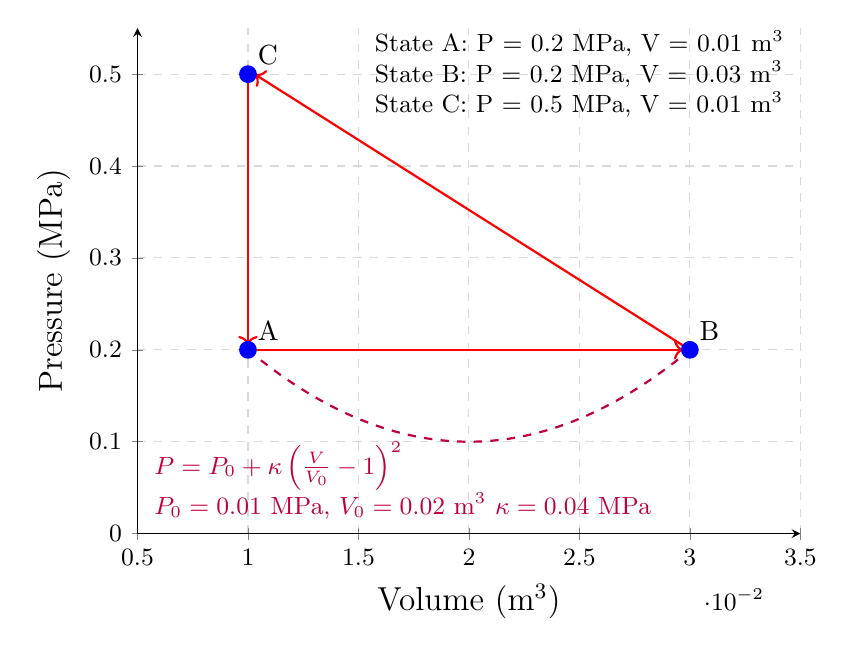
\begin{tikzpicture}
  \begin{axis}[
      xlabel={Volume (m$^3$)},
      ylabel={Pressure (MPa)},
      xmin=0.005, xmax=0.035,
      ymin=0.00, ymax=0.55,
      grid=major,
      grid style={dashed, gray!30},
      axis lines=left,
      width=10cm,
      height=8cm,
      tick label style={font=\small},
      label style={font=\large}
    ]

    % Define the three states
    \coordinate (A) at (0.01, 0.2);
    \coordinate (B) at (0.03, 0.2);
    \coordinate (C) at (0.01, 0.5);

    % Plot the points
    \addplot[only marks, mark=*, mark size=3pt, blue] coordinates {
      (0.01, 0.2)  % Point A
      (0.03, 0.2)  % Point B
      (0.01, 0.5)  % Point C
    };

    % Add labels for the points
    \node[above right] at (A) {A};
    \node[above right] at (B) {B};
    \node[above right] at (C) {C};

    % Draw arrows between states
    % Arrow A to B (horizontal, constant pressure)
    \draw[->, thick, red] (0.01, 0.2) -- (0.0297, 0.2);

    % Arrow B to C (vertical line, then to C)
    \draw[->, thick, red] (0.03, 0.2) -- (0.0103, 0.5);

    % Arrow C to A (vertical, constant volume)
    \draw[->, thick, red] (0.01, 0.5) -- (0.01, 0.205);

    % Add state information as text
    \node[align=left, font=\small] at (0.025, 0.5) {
      State A: P = 0.2 MPa, V = 0.01 m$^3$ \\
      State B: P = 0.2 MPa, V = 0.03 m$^3$ \\
      State C: P = 0.5 MPa, V = 0.01 m$^3$
    };

    % Plot the equation P = P_0 + κ(V/V_0 - 1)^2
    % where P_0 = 0.01 MPa, V_0 = 0.02 m^3, κ = 0.04 MPa
    \addplot[domain=0.01:0.03, samples=100, dashed, thick, purple]
    {0.1 + 0.4*((x/0.02) - 1)^2};

    % Add equation label
    \node[align=left, font=\small, purple] at (0.017, 0.058) {
      $P = P_0 + \kappa\left(\frac{V}{V_0} - 1\right)^2$ \\
      $P_0 = 0.01$ MPa, $V_0 = 0.02$ m$^3$ $\kappa = 0.04$ MPa
    };

  \end{axis}
\end{tikzpicture}

      \vspace{0.5em}
      \captionof{figure}{PV diagram of three states with arrows
      indicating state changes.}
    }

    \begin{enumerate}[(a)]
      \item Calculate $Q$ and $W$ for the process taking state A to
        state B along a straight path

        \boxedanswersmall{
          \begin{align*}
            dU &= \overbrace{TdS}^{Q} - \overbrace{PdV}^{W} + \delta W' \\
            & \delta W' = 0 \\
            W &= PdV \\
            &
            \begin{aligned}
              P &= \SI{0.2}{\mega\pascal} \\
              dV &= \SI{0.03}{\meter\cubed} - \SI{0.01}{\meter\cubed} \\
              dV &= \SI{0.02}{\meter\cubed}
            \end{aligned} \\
            W &= (\SI{0.2e6}{\pascal})(\SI{0.02}{\meter\cubed}) \\
            \Aboxed{W &= \SI{4000}{\joule}} \\
            \Delta U &= Q + W \\
            Q &=\delta U - W \\
            &
            \begin{aligned}
              \Delta U &= U_2 - U_1 \\
              U &= U_0 + 5 PV \\
              &
              \begin{aligned}
                U_2 &= U_0 + 5
                (\SI{0.2}{\mega\pascal})(\SI{0.03}{\meter\cubed}) \\
                U_1 &= U_0 + 5
                (\SI{0.2}{\mega\pascal})(\SI{0.01}{\meter\cubed}) \\
              \end{aligned} \\
              \Delta U &=
              5(\SI{0.2e6}{\pascal})(\SI{0.03}{\meter\cubed} -
              \SI{0.01}{\meter\cubed}) \\
              \Delta U &=\SI{20000}{\joule} \\
            \end{aligned} \\
            Q &= (\SI{20000}{\joule}) - (\SI{4000}{\joule}) \\
            \Aboxed{Q &= \SI{16000}{\joule}}
          \end{align*}
        }

      \item Calcualte $Q$ and $W$ for the process taking state B to
        state C along a straight path

        \boxedanswer{
          \begin{align*}
            \text{no clue lol}
          \end{align*}
        }

      \item Calculate $Q$ and $W$ for the process taking state C to
        state A along a straight path

        \boxedanswer{
          Because there is no change in volume, no work is being done.

          \begin{align*}
            W &= P\overbrace{dV}^{0} \\
            \Delta U &= Q + \cancel{W} \\
            Q &= \Delta U  = U_2 - U_1\\
            &
            \begin{aligned}
              \Delta U &= 5V(P_2 - P_1) \\
              \Delta U &=
              5(\SI{0.01}{\meter\cubed})(\SI{0.5}{\mega\pascal} -
              \SI{0.1}{\mega\pascal}) \\
              \Delta U &= \SI{20000}{\joule}
            \end{aligned} \\
            \Aboxed{Q &= \SI{20000}{\joule}} \\
            \Aboxed{W &= \SI{0}{\joule}}
          \end{align*}
        }

      \item Calculate $Q$ and $W$ for the process taking state A to
        state B along the parabolic path $P = P_0 +
        \kappa\left(\frac{V}{V_0} - 1\right)^2$ where
        $P_0 = \SI{0.01}{\mega\pascal}, V_0 = \SI{0.02}{\meter\cubed}$, and
        $\kappa = \SI{0.04}{\mega\pascal}$.
    \end{enumerate}
  \item  {[35 pts]} Consider an isolated system (no heat, matter, or
    work may cross the system boundary)
    consisting of three internal compartments A, B, and C.
    Compartment A is 1 liter, B is 2 liters, and
    C is 4 liters. The compartments are separated by partitions; each
    partition has a valve (V1 and V2)
    which may be opened remotely. Initially the central volume (B) is
    filled with an ideal gas at 298K and
    \SI{354.6}{\kilo\pascal} and the other two (A and C) are
    completely evacuated (i.e., \SI{0}{\pascal}).

    \begin{figure}[ht]
      \centering
      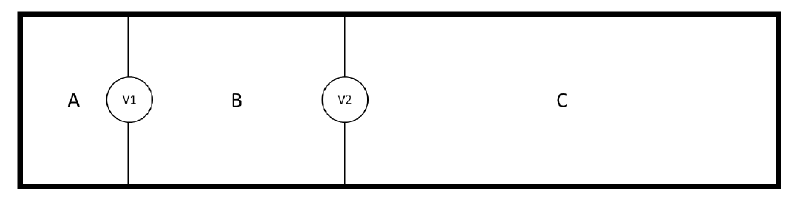
\includegraphics[width=0.6\textwidth]{./assets/q_4_fig.png}
    \end{figure}

    \begin{enumerate}[(a)]
      \item Consider the following processes:

        \textit{First process: The valve to the A side is opened, the gas
          expands freely into compartment A, and
          the system comes to equilibrium. Then the valve to the C side
          is opened, and the system comes
        to equilibrium again.}

        \hspace{0.5 cm}

        \textit{Second process: Both valves are opened simultaneously, the
          gas expands freely into both compart-
        ments, and the A/B/C system comes to equilibrium.}

        \hspace{0.5 cm}

        Which of the processes above produces more entropy? You must
        explain your answer completely.

      \item  The internal energy of an ideal gas is determined solely
        by its temperature. If that’s the case,
        what is the final temperature of the system in the first process?

      \item It is found that the change in entropy of the first
        process is \SI{5.5}{\joule\per\kelvin}. What can you say about
        the reversibility of the process?
    \end{enumerate}

  \item {[15 pts]}
    \begin{enumerate}[(a)]
      \item If $\psi(m) = z − mx$ is the Legendre
        transform of $z(x)$ (where $m$ is conjugate to $x$), prove
        that
        \[\frac{d^2\psi}{dm^2} = -\left[\frac{d^2z}{dx^2} \right]^{-1}\]

        Hint: the chain rule will come in handy,
        as will the identity
        $dx/dz = 1/(dz/dx)$.

      \item Describe what this implies for the graph of $\psi$
        relative to the graph of $z$.
    \end{enumerate}

\end{enumerate}

\end{document}
